\begin{qBox}{1}
Plot \( \langle M \rangle \) vs \( T \) for and compare with the results from the 
text and lecture.

\tcblower

Below are the images from lecture and the text, respectively:

\begin{figure}[H]
    \centering
    \begin{minipage}{0.45\linewidth}
        \centering
        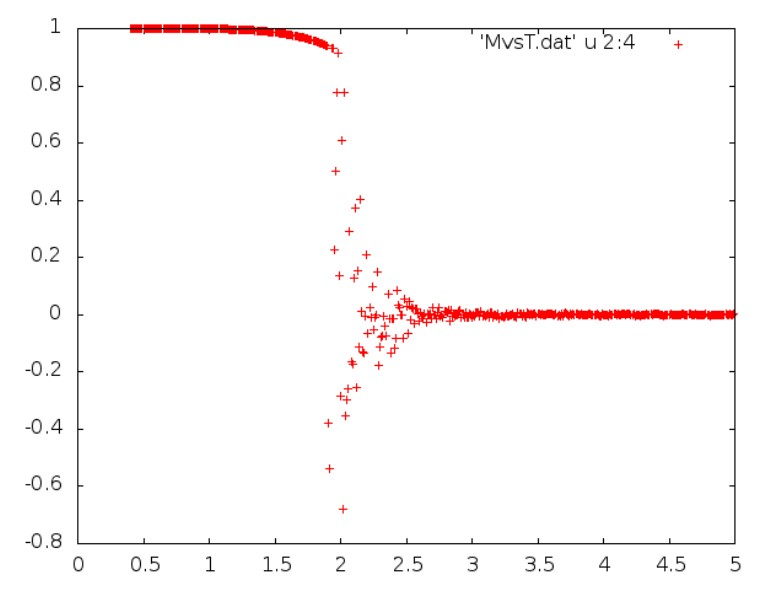
\includegraphics[ width = 0.95\linewidth ]{figures/1_lecture.jpg}
        \caption{The plot from lecture}
    \end{minipage}%
    \begin{minipage}{0.45\linewidth}
        \centering
        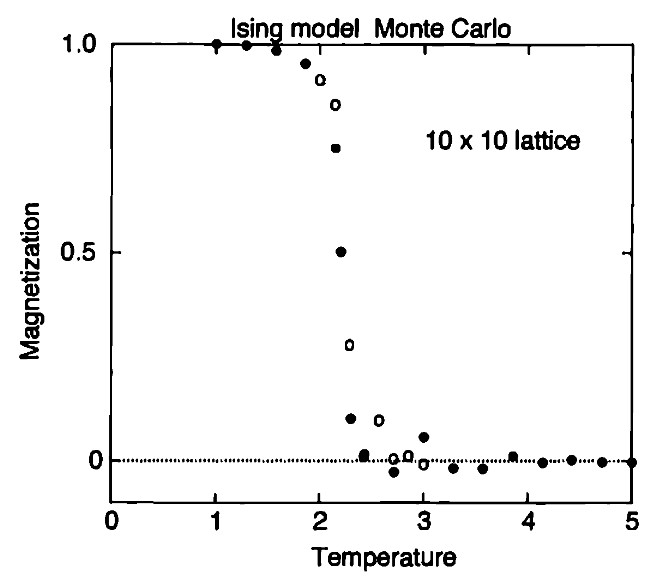
\includegraphics[ width = 0.95\linewidth ]{figures/1_text.jpg}
        \caption{The plot from the text}
    \end{minipage}%
\end{figure}

Below are the images that I was able to produce (both coarse and fine):

\begin{figure}[H]
    \centering
    \begin{minipage}{0.45\linewidth}
        \centering
        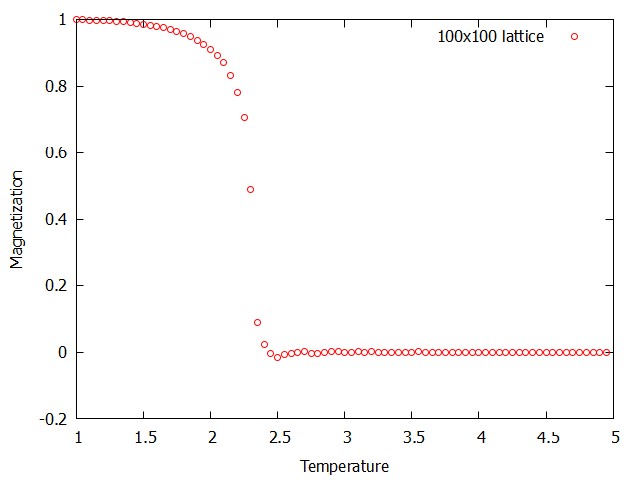
\includegraphics[ width = 0.95\linewidth ]{figures/assignment6_1.png}
        \caption{The coarse plot}
    \end{minipage}%
    \begin{minipage}{0.45\linewidth}
        \centering
        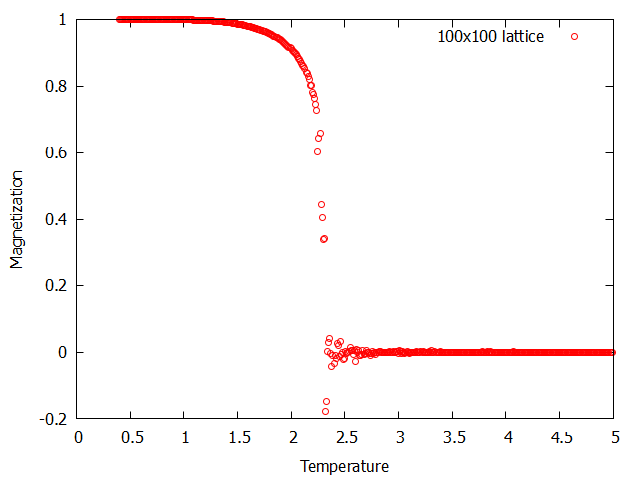
\includegraphics[ width = 0.95\linewidth ]{figures/assignment6_1_fine.png}
        \caption{The fine plot}
    \end{minipage}%
\end{figure}

From my plots, we can see that the magnetization stays around \( 1 \) at lower 
temperatures (e.g., \( T < 1 \)) and \( 0 \) around higher temperatures 
(e.g., \( T > 2.5 \)). 
As the temperature approaches \( \approx 2.27 \), we can see that the magnetization 
drops very steeply and the plot resembles very closely to that of a waterfall.
I.e., near the critical temperature \( T_{ C } \), we have very large fluctuations with 
the magnetization.
This makes sense to see as the text notes that a system at its critical point is 
extremely sensitive to small perturbations; thus, we should expect to see large
fluctuations around \( T_{ C } \). 

\baseSkip

Furthermore, we see that the fluctuations around \( T_{ C } \) in the plot given in 
lecture are much larger than what we observed, and our plot resembled the one given 
in the text much more closely.
I think that this is most likely due to the fact that I reduced the number of Monte 
Carlo steps (I brought it all the way down to \( 2000 \) to save time, which is much 
closer to the \( 1000 \) that the text used), which essentially means that the system 
had less time to evolve. 
\end{qBox}